  \documentclass[12pt]{article}
 
\usepackage[margin=1in]{geometry}
\usepackage{amsmath,amsthm,amssymb}
\usepackage[spanish]{babel}
\decimalpoint
\usepackage[utf8]{inputenc}
\usepackage{enumitem, kantlipsum}
\usepackage{graphicx}
\newcommand{\angstrom}{\mbox{\normalfont\AA}}
\setlength{\parindent}{0cm} 

\begin{document}
 
\begin{center}
\Large \textbf{C.Física Moderna: Solución Taller 8}\\
\normalsize \textbf{Longitud de onda de De-Broglie, experimento de Davisson-Germer y de Frank-Hertz}
\end{center}
 
  

\section{Longitud de onda de De-Broglie }



\begin{enumerate}
	\item Calcule la longitud de onda de De-Broglie de un cuerpo de masa 100 kg moviéndose a $0.5c$.
	\item Calcule la longitud de onda de De-Broglie de un electrón que es acelerado por una diferencia de potencial de 5V.
	\item Compare las longitudes de onda obtenidas y concluya sobre la longitud de onda para objetos macroscópicos.
\end{enumerate}


\begin{center}
	\textbf{Solución}
\end{center}

1. Para la longitud de onda de De-Broglie se requiere el momento, que es:

\begin{equation*}
p = \frac{m v}{\sqrt{1-\frac{v^2}{c^2}}}
\end{equation*} 

La longitud de onda se obtiene dividiendo $h$ sobre el momento calculado:

\begin{align*}
\lambda &= \frac{h}{p} \\
&= \frac{h\sqrt{1-\frac{v^2}{c^2}}}{m v}\\
& = 3.83 \times 10^{-44} \text{m}
\end{align*}

2. Se plantea la conservación de energía para despejar el momento.
\begin{equation*}
\frac{p^2}{2m} = q V
\end{equation*}

Despejando el momento y usando la ecuación de De-Broglie:

\begin{align*}
\lambda &= \frac{h}{\sqrt{2 m q V}}\\
 &= 2.24 \times 10^{-11} \text{m}
\end{align*}

3. La longitud de onda macroscópica es demasiado pequeña para ser observada.


\noindent\rule{16.5cm}{0.4pt}





\section{Experimento de Davisson-Germer}

 En el experimento de Davisson-Germer se aceleran electrones mediante un potencial $V$, y luego
se hace incidir estos electrones sobre un cristal. Dado que la longitud de onda asociada de Broglie de los
electrones es del orden de la longitud de separación de los planos del cristal, los electrones son
difractados.

\begin{enumerate}
	\item Encuentre  la relación entre las posiciones donde se detecta una mayor intensidad de electrones
	detectados y el voltaje de aceleración.
	\item Para un voltaje de aceleración de 54 V, establezca la primera posición donde se detectará una
	mayor intensidad de electrones para un cristal con distancia interplanar de 0.092 nm.
\end{enumerate}


\begin{center}
	\textbf{Solución}
\end{center}


1. De la conservación de energía se obtiene el momento del electrón incidente.

\begin{equation*}
\frac{p^2}{2m} = q V
\end{equation*}

 Este momento se usa para calcular su longitud de onda de De-Broglie.

\begin{equation*}
\lambda = \frac{h}{p} = \frac{h}{\sqrt{2 m q V}}
\end{equation*}

La longitud de onda se reemplaza en la ley de Bragg:

\begin{equation}
n\lambda = 2 d \sin\theta
\end{equation}

Y se despeja el ángulo:

\begin{equation}
\sin\theta =   \frac{nh}{2d\sqrt{2 m q V}}
\end{equation}


2. Utilizando $d=0.092$ nm y $n=1$ obtenemos el ángulo:

\begin{equation*}
\theta = 62.2^{\circ}
\end{equation*}

\noindent\rule{16.5cm}{0.4pt}

\section{Experimento de Frank-Hertz}

En el experimento de Frank-Hertz se hace fluir corriente eléctrica sobre un tubo que contiene
vapor de mercurio, el nivel de corriente se controla con un voltaje variable de aceleración entre el
cátodo A y una rejilla, la corriente se mide entre la rejilla y el cátodo B, en el cual se mantiene un
pequeño voltaje de frenado constante. La gráfica de corriente versus voltaje en el tubo, se muestra
a continuación, donde se muestra una caída abrupta de la corriente para 4.9 V, 9.8 V, 14.7 V.

	\begin{figure}[h!]
		\centering
	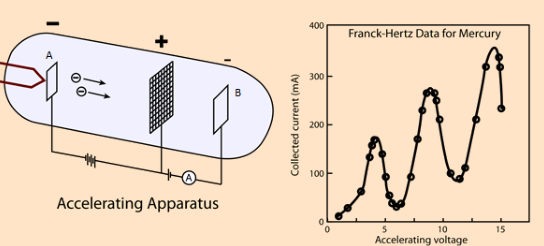
\includegraphics[scale=1, angle=0]{frank}
	\caption{Figuras tomadas de HyperPhysics}
\end{figure}

\begin{enumerate}
	\item Explicar en términos de colisiones elásticas e inelásticas entre los electrones y los átomos de
	mercurio el resultado de esta gráfica.
	\item  Determinar frecuencia y longitud de onda de la radiación electromagnética emitida por el átomo
	de mercurio para la transición entre el estado base y el primer nivel de energía.
	\item Suponga que se llena ahora el tubo con hidrógeno. ¿Para qué voltaje de aceleración espera que la
	corriente caiga de forma abrupta?
\end{enumerate}


\begin{center}
	\textbf{Solución}
\end{center}

1. Al aumentar el voltaje de aceleración, la corriente sobre el gas aumenta ya que los electrones sufren una colisión elástica con los atomos de mercurio. En ese proceso los electrones no pierden casi energía. Solo cuando se llega a las corrientes donde los electrones tienen la energía para excitar el mercurio, los electrones colisionan inelásticamente con el mercurio cediéndole toda su energía. Esto causa que la corriente caiga ya que la energía que pierden los electrones con los átomos de mercurio es irradiada y no se retorna a los electrones.\\

2. La energía para excitar el átomo de mercurio de su estado base a su primer estado excitado es 4.9V por la carga del electrón. Es decir que el átomo emitido al volver a su estado basal tendrá dicha energía. Podemos encontrar la frecuencia de un fotón con su energía:

\begin{align*}
f = \frac{qV}{h} = 1.18 \times 10^{15} \;\text{Hz}
\end{align*}

Y su longitud de onda:

\begin{equation*}
\lambda = \frac{hc}{qV} = 253 \;\text{nm}
\end{equation*}

3. Calculamos la diferencia entre los dos primeros niveles de energía:

\begin{equation*}
\Delta E = E_1 - E_2 = 10.2 \text{eV}
\end{equation*}

El voltaje entonces sera:

\begin{equation*}
V = \frac{\Delta E}{e} = 10.2 \text{V}
\end{equation*}


Donde $e$ es la carga de un electrón.

\noindent\rule{16.5cm}{0.4pt}








\begin{center}
	\textbf{Fórmulas útiles}
\end{center}

Longitud de onda de De-Broglie:

\begin{equation*}
\lambda = \frac{h}{p}
\end{equation*}

Ley de Bragg:

\begin{equation}
n\lambda = 2 d \sin\theta
\end{equation}

Energías permitidas del átomo de hidrógeno:

\begin{equation*}
E_n = - \frac{13.6}{n^2} \text{eV}
\end{equation*}


\end{document}